\let\negmedspace\undefined
\let\negthickspace\undefined
\documentclass[journal]{IEEEtran}
\usepackage[a4paper, margin=10mm, onecolumn]{geometry}
%\usepackage{lmodern} % Ensure lmodern is loaded for pdflatex
\usepackage{tfrupee} % Include tfrupee package

\setlength{\headheight}{1cm} % Set the height of the header box
\setlength{\headsep}{0mm}  % Set the distance between the header box and the top of the text

\usepackage{gvv-book}
\usepackage{gvv}
\usepackage{cite}
\usepackage{amsmath,amssymb,amsfonts,amsthm}
\usepackage{algorithmic}
\usepackage{graphicx}
\usepackage{float}
\usepackage{textcomp}
\usepackage{xcolor}
\usepackage{txfonts}
\usepackage{listings}
\usepackage{enumitem}
\usepackage{mathtools}
\usepackage{gensymb}
\usepackage{comment}
\usepackage[breaklinks=true]{hyperref}
\usepackage{tkz-euclide} 
\usepackage{listings}
% \usepackage{gvv}                                        
\def\inputGnumericTable{}                                 
\usepackage[latin1]{inputenc}                                
\usepackage{color}                                            
\usepackage{array}                                            
\usepackage{longtable}                                       
\usepackage{calc}                                             
\usepackage{multirow}                                         
\usepackage{hhline}                                           
\usepackage{ifthen}                                           
\usepackage{lscape}
\usepackage{tikz}
\usetikzlibrary{patterns}

\begin{document}

\bibliographystyle{IEEEtran}
\vspace{3cm}

\title{12.180}
\author{ee25btech11063-vejith}

\maketitle
% \maketitle
% \newpage
% \bigskip
{\let\newpage\relax\maketitle}
\renewcommand{\thefigure}{\theenumi}
\renewcommand{\thetable}{\theenumi}
\setlength{\intextsep}{10pt} % Space between text and floats
\textbf{Question}\\
The system of linear equations\\
\hspace*{3cm}4x+2y=7\\
\hspace*{3cm}2x+y=6  has 
\begin{multicols}{2}
\begin{enumerate}[label=\alph*)]
    \item a  unique solution
    \item no solution
    \item infinite number of solutions
    \item exactly two distinct solutions 
\end{enumerate}
\end{multicols}

\textbf{solution}:\\
Given linear equations are
\begin{align}
    \brak{4\hspace{0.5cm} 2}\myvec{x\\y}=7\\
     \brak{2\hspace{0.5cm} 1}\myvec{x\\y}=6
\end{align}
Equations (1) and (2) can be written as
\begin{align}
    \begin{pmatrix}
        4 & 2\\
        2 & 1
    \end{pmatrix} \myvec{x\\y}=\myvec{7\\6}
\end{align}
Forming the augmented matrix
\begin{align}
     \left(\begin{array}{cc|c}
        4 & 2 & 7 \\
        2 & 1 & 6 
\end{array}\right) &\xleftrightarrow{R_2 \rightarrow R_2- \frac{1}{2} \times R_1}  \left(\begin{array}{cc|c}
        4 & 2 & 7 \\
        0 & 0 & \frac{5}{2} 
\end{array}\right)
\end{align}
As in the augmented matrix the entries of second  row are 0 their linear combination should also give 0 but it is  $\frac{5}{2}$ which is a contradiction\\
$\implies$ So,the given system of linear equations has no solution
\begin{figure}
    \centering
    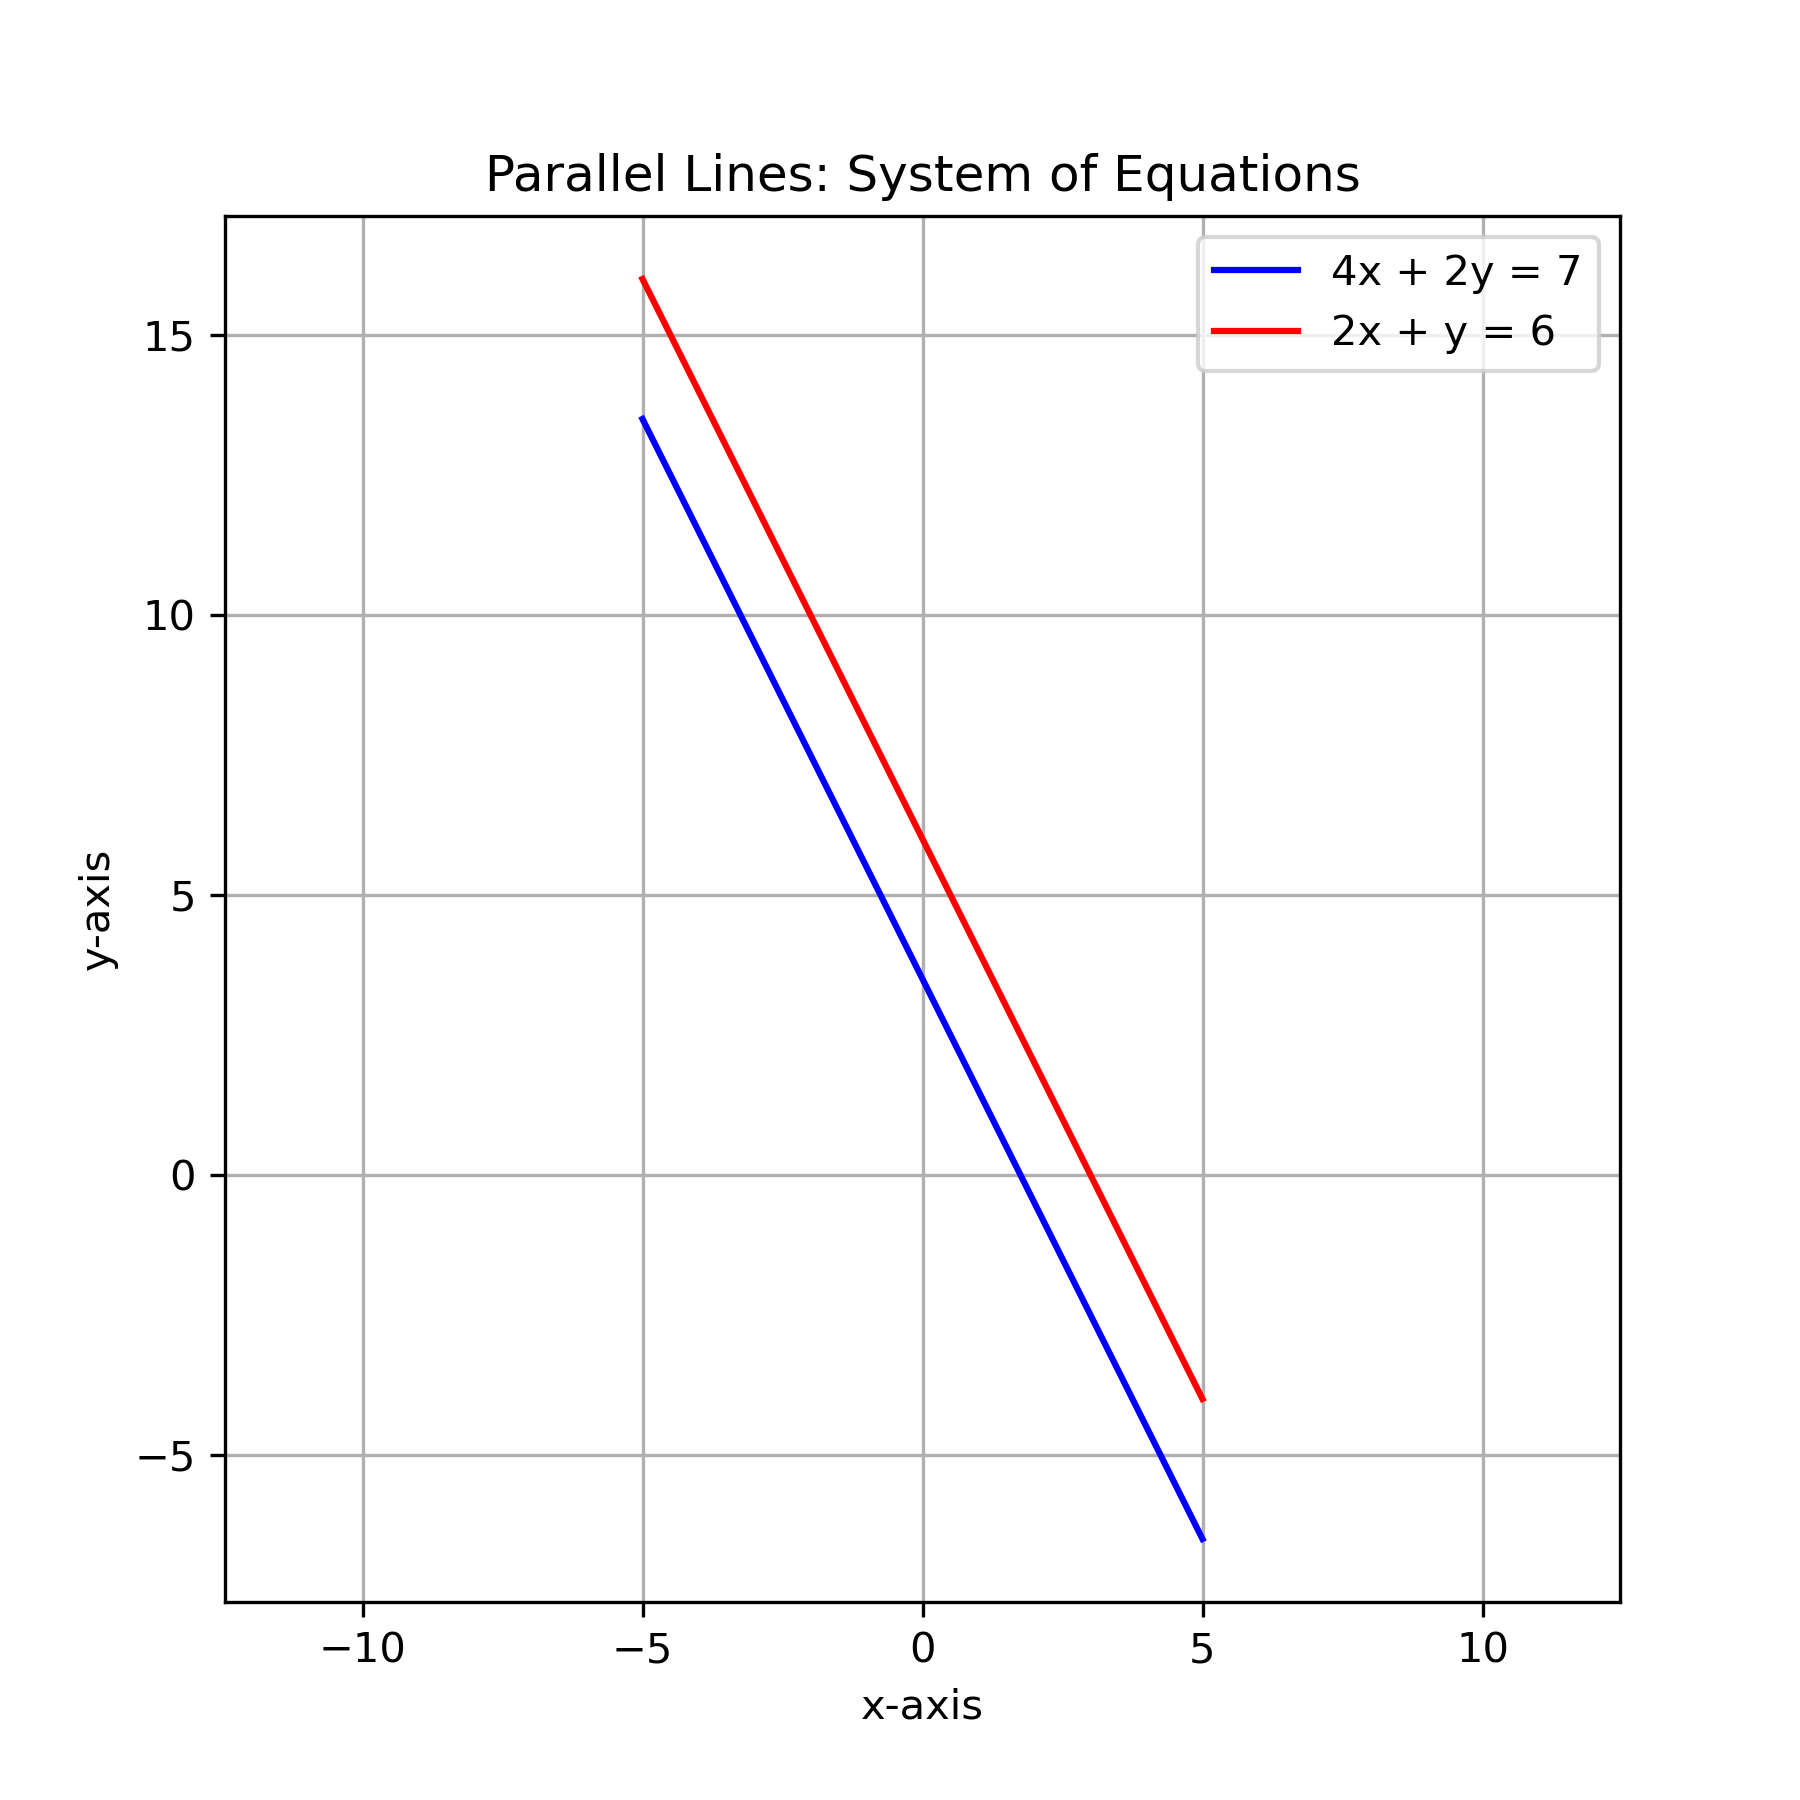
\includegraphics[width=0.54\columnwidth]{figs/01.png}
    \caption{}
    \label{fig:placeholder}
\end{figure}
\end{document}
